% !TEX root =  ThesisMaster.tex

\chapter{Semi-monotonic programs}
	\label{CH_03}
% should use past tense

In this chapter we describe our discovery that if the test program $P$ meets a certain property that we call semi-monotonicity, then we can use a different wrapping loop. 
%and greatly reduce the time Getafix and jMoped needs to check for reachability.

\section{Discovery by mistake}
During the initial tests with the sanity check program of bit length 32, the program terminates in less than a minute and gives the correct output count. Later we time the execution of an empty loop from $0$ to $2^{32} - 1$ and the result is $10.30$ seconds, so theoretically the double loop would take a much longer time to terminate, longer than our test result with sanity check.  Listing \ref{lst:1stTry} shows the C code we used. We set base to 0 in our tests.

\lstset{language=C}  
\begin{lstlisting}[float=!h, caption={Initial implementation of the double loop with sanity check in C.},label=lst:1stTry]
uint32_t S = 0;
uint32_t O = 0;
uint32_t SMax = S - 1;
uint32_t OMax = O - 1;
uint32_t OCounter = 0;
uint32_t OTemp = 0;
uint32_t base = 0;
for (;O<OMax;O++){
	for (;S<SMax;S++){
		//program start here
		if (S < 16)
			OTemp = base + S;
		else
			OTemp = base;
		//program end here
		if (OTemp == O){
			OCounter ++;
			break;
}	}	}
\end{lstlisting}

Due to the large difference in actual execution time and the theoretical time, we decided to inspect the code for errors. Our code differs from Algorithm \ref{alg:doubleLoop} at two places: First, $S$ and $O$ can not reach $SMax$ and $OMax$ due to the use of $<$, thus the upper bound is not tested. Second, in the inner loop, we did not initialize $S$ to $0$ except for its first iteration. The first point does not affect the output count of the sanity check example as every $S$ greater than $16$ will lead to a $P(S)$ value of $base$ which is $0$. The second point is the cause of the large time difference, because essentially $P$ only executes once for each $S$, reaching a total of $2^{32}$ times, much smaller than the full double loop in which $P$ executes $2^{2 \times 32}$ times.

We found that removing the initialization of $S$ to $0$ can be a way to speed up some programs, but not all. 
Specifically, program $P$ has to obey certain properties in order for this initialization to give an accurate answer:

\begin{enumerate}
\item Function $P$ is monotonically increasing within range $[0, n]$.
\item The output of function $P$ with $S$ in range $[0, n]$ has to start with zero and is continuous.
\item Each output of function $P$ with $S$ in range $[n+1, 1\ll bitLength-1]$ can be produced by at least one $S$ in range $[0, n]$.
\end{enumerate}

Figure \ref{fig:1stTry} shows an example function that follows these properties. In the first part $[0, 4]$, function output has to start from $0$ and be continuously increasing. As to the second part $[5, 6]$, each output has to be equal to an output in $[0, 4]$.

\begin{figure}
\centering
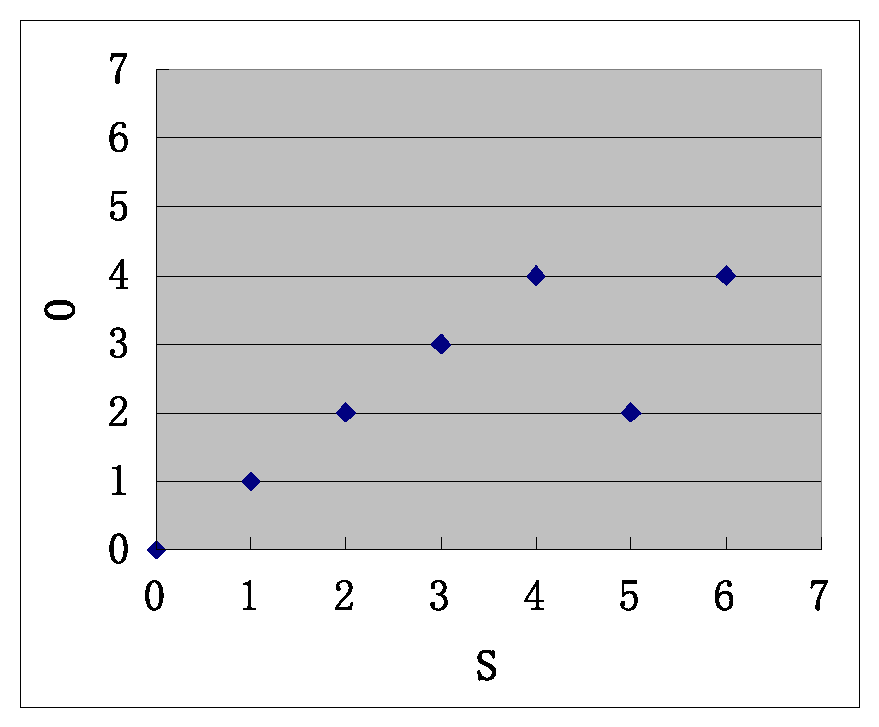
\includegraphics[scale=0.8]{Figures/1stTry}
\caption{A function that follows the properties from the first optimization.}
\label{fig:1stTry}
\end{figure}

\section{Improvements}
The properties that $P$ has to follow in order for the optimization to work is rather strict. For example in the sanity check test, the optimization only works when $base$ is $0$. A possible solution would be to start $O$ at the lowest value $P$ can output, in essence pulling the function down on $y$ axis so that it starts with $0$. However, this approach does not ease the restrictions.

In our second attempt as shown in Listing \ref{lst:2ndTry} to improve this optimization method, we started with monotonicity and rearranged the architecture of the outer program. The problem is to count the number of outputs of a monotonically increasing function, and our solution is to iterate through the entire range of $S$ and keep track of the highest output value. If $P$ generates a value $OOut$ which is larger than the current largest value, then $OOut$ replaces that value and $OCounter$ increases. The properties that $P$ has to follow in order to use this optimization is different from the first one.

For program $P$, it has to follow either of the following conditions:
\begin{enumerate}
\item $P_{func}(s) \geq \max_{ s'\leq s}{P_{func}(s')}$
\item $P_{func}(s) \in \set{P_{func}(s') \mathbin{|} s'\leq s}$
\end{enumerate}
To enable the optimization.

\begin{figure}
\centering
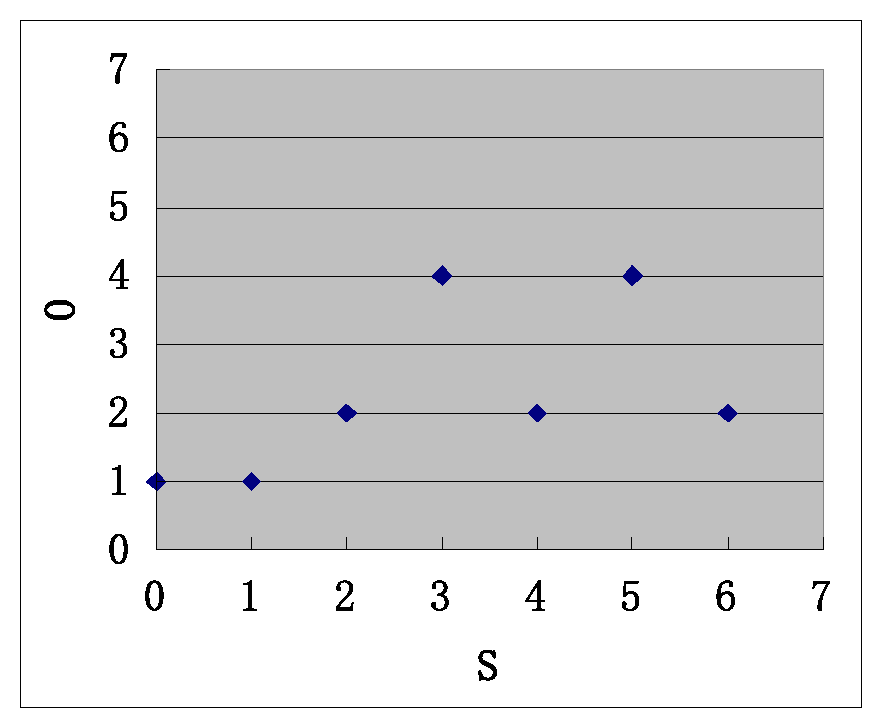
\includegraphics[scale=0.8]{Figures/2ndTry}
\caption{A function that follows the properties from the second optimization.}
\label{fig:2ndTry}
\end{figure}

Also Figure \ref{fig:2ndTry} shows an example function that follows these conditions. A new output value has to be either larger than all previous values like when $S$ is $3$, or is within the set of all previous outputs like when $S$ is $6$.



So with the second attempt, we removed the requirement for $P$ to be continuous and start with $0$ from the first attempt. The execution time for the optimization is $2^{bitLength} \times t(P)$, which is $1/2^{bitLength}$ of the execution time of the original double loop.


\lstset{language=C}  
\begin{lstlisting}[float=!h, caption={Implementation of the optimization with sanity check in C.},label=lst:2ndTry]
unsigned int S = 0;
unsigned int SMax = 4294967295;
unsigned int base =4;
unsigned int STemp = S;
unsigned int OTemp = 0;
//program starts here
if (STemp< 16){OTemp = base+ STemp;}
else{OTemp = base;}
//program ends here
unsigned int OCounter = 1;
unsigned int OMax = OTemp;
S++; 
while (S<= SMax){
	STemp = S;
	//program starts here
	if(STemp < 16){OTemp = base+ STemp;	}
	else{OTemp = base;}
	//program ends here
	if (OTemp > OMax ){
		OMax = OTemp;
		OCounter= OCounter+1;
	}
	if(S < SMax) S=S+1;
	else break;
}
\end{lstlisting}
